\documentclass[aspectratio=169,10pt]{beamer}
\usetheme{metropolis}
\metroset{sectionpage=none}
\usepackage[utf8]{inputenc}
\usepackage{booktabs}
\usepackage{array}
\usepackage{amsmath,amssymb}
\usepackage{graphicx}
\usepackage{xcolor}
\newcommand{\xiref}{\xi_{\mathrm{ref}}}
\setbeamertemplate{frame footer}{RL setup optimisation -- progress, 26 Oct -- 2 Nov 2026}

\title{Reward engineering, simulator fidelity and lap-time benchmarks}
\subtitle{RL driving agent in OCD: Barcelona and Shanghai}
\author{Ibrahim Khaled}
\date{2 November 2026}

\begin{document}

% 1
\maketitle

% 2 ------------------------------------------------------------------
\begin{frame}[shrink=9]{Reward: from line tracking to time-optimal}
  \small
  \textbf{Old} (\texttt{ref\_tracking}), per 50\,Hz tick, $e$ = offset to the reference line $\xiref$:
  \[
    r = a\,\Delta s - b\,\Delta t\,\bigl(1 + \underbrace{\dot u^\top W \dot u}_{\text{jitter}}\bigr) - \underbrace{c\,e^2}_{\text{tracking}},
    \qquad P_{\text{fail}} = 50 + 30\,c\,e_{\text{exit}}^2
  \]
  \textbf{New} (\texttt{time\_pbrs}, R1):
  \[
    r = a\,\Delta s - b\,\Delta t + \bigl[\gamma\,\Phi(s') - \Phi(s)\bigr],
    \qquad \Phi(s) = -k\,|e(s)|,\; k = 1\,\text{m}^{-1},\qquad P_{\text{fail}} = 100
  \]
  \vspace{-10pt}
  \begin{columns}[T]
    \begin{column}{0.62\textwidth}
      \begin{enumerate}
        \item \textbf{Jitter term removed} (logged only): top racing agents (Linesight, GT Sophy) use none.
        \item \textbf{Linear $|e|$, not $e^2$}: constant gradient instead of flat-then-explosive.
        \item \textbf{Potential-based shaping} (Ng 1999): cannot change the optimal driver; $\xiref$ only guides early learning.
      \end{enumerate}
      Old problem: tracking cost (175.9) exceeded lap time (123.3); the driver stayed glued to a \emph{safe} line.
    \end{column}
    \begin{column}{0.36\textwidth}
      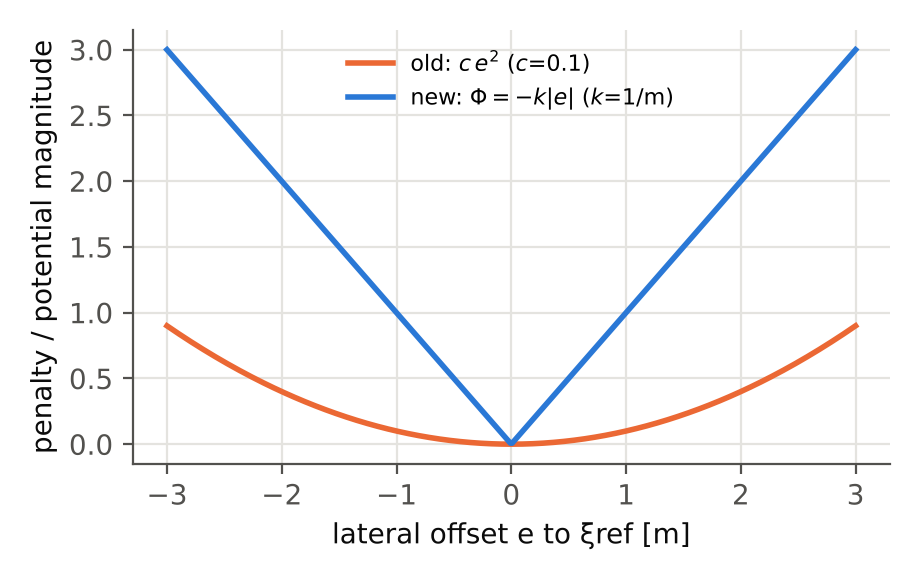
\includegraphics[width=\linewidth]{fig/penalty_shape.png}
    \end{column}
  \end{columns}
\end{frame}

% 3 ------------------------------------------------------------------
\begin{frame}{Effect of the new reward (Shanghai)}
  \centering
  \begin{tabular}{@{}llrr@{}}
    \toprule
    Run & Car / reward & Best clean lap 2 & Own QSS (safe line)\\
    \midrule
    full1 & AV-21, old reward & 122.85\,s & 133.9\,s\\
    r1\_warm & AV-21, new reward, warm start & 123.04\,s & 133.9\,s\\
    sf70h\_mac\_r1 & sf70h\_tum, new reward, from scratch & \textbf{103.24\,s} & 104.78\,s\\
    p1\_TUM & sf70h\_tum + TUM-like setup, new reward & \textbf{101.27\,s} & 103.56\,s\\
    \bottomrule
  \end{tabular}
  \bigskip
  \raggedright
  \begin{itemize}
    \item The warm start kept the old line-following habits and gained nothing.
    \item From scratch, the free driver \textbf{beats the QSS lap on its own safe line} by 1.5--2.3\,s, because it is no longer tied to that line.
    \item Cost: a lower clean rate (48/194 clean deterministic evaluations in sf70h\_mac\_r1).
  \end{itemize}
\end{frame}

% 4 ------------------------------------------------------------------
\begin{frame}{Vehicle dynamics: three cars, built in layers}
  \footnotesize
  \renewcommand{\arraystretch}{1.05}
  \begin{tabular}{@{}>{\raggedright\arraybackslash}p{0.17\textwidth}>{\raggedright\arraybackslash}p{0.24\textwidth}>{\raggedright\arraybackslash}p{0.26\textwidth}>{\raggedright\arraybackslash}p{0.26\textwidth}@{}}
    \toprule
    & \texttt{av21} (shipped OCD) & \texttt{sf70h\_tum} (27 Oct) & \texttt{sf70h\_f1} (1 Nov)\\
    \midrule
    Idea & Dallara AV-21 (Indy Autonomous Challenge) & AV-21 model with every value TUM's \texttt{F1\_Shanghai.ini} gives & \texttt{sf70h\_tum} + F1 values from papers and the FIA rules\\
    Mass, geometry, aero & AV-21 (800\,kg, 3.2\,m) & TUM (733\,kg, 3.6\,m) & TUM\\
    Tyre peak $\mu$ & AV-21 (1.46 / 1.16) & TUM (1.65--2.15) & TUM\\
    Tyre slip stiffness, shape & AV-21 & \leavevmode\alert{AV-21} & PL14 (Limebeer)\\
    Inertias & AV-21 & scaled ($I \propto mL^2$) & scaled\\
    Steering lock & 0.6\,rad & \leavevmode\alert{0.6\,rad} & 0.30\,rad\\
    Heave springs & off & off & 1.0 / 0.25\,MN/m\\
    Brakes & 12\,kN\,m, 0.50 & 12--15\,kN\,m, 0.50 & 15\,kN\,m, 0.58\\
    Footprint & 4.2\,$\times$\,2.0\,m & 4.6\,$\times$\,2.0\,m & 5.006\,$\times$\,2.07\,m\\
    \bottomrule
  \end{tabular}
  \smallskip

  Each car is opt-in; \texttt{av21} and \texttt{sf70h\_tum} stay bit-identical (85 unit tests, Shanghai \texttt{lap.csv} sha256 unchanged).
\end{frame}

% 5 ------------------------------------------------------------------
\begin{frame}{\texttt{sf70h\_tum}: an F1-like car from TUM's open data}
  \begin{columns}[T]
    \begin{column}{0.46\textwidth}
      \small
      \begin{tabular}{@{}lll@{}}
        \toprule
        & AV-21 & \texttt{sf70h\_tum}\\
        \midrule
        Mass & 800\,kg & 733\,kg\\
        Wheelbase & 3.2\,m & 3.6\,m\\
        Tyre grip (peak $\mu$) & 1.2--1.5 & 1.65--2.15\\
        Engine & TUM F1 & TUM F1\\
        Aero (downforce, drag) & TUM F1 & TUM F1\\
        \bottomrule
      \end{tabular}
    \end{column}
    \begin{column}{0.52\textwidth}
      \begin{itemize}
        \item Source: TUM's open F1 car file (\texttt{F1\_Shanghai.ini}, laptime-simulation). Every value it provides was copied; the rest stayed AV-21.
        \item Biggest change: \textbf{tyre grip at F1-slick level} (about 50\,\% more than the AV-21 on average).
        \item \textbf{ERS and DRS were added to the model but are OFF in every RL run} and in our comparisons. Only TUM's 91.24\,s reference uses them.
        \item Brakes raised from 12 to 15\,kN\,m so the F1 grip can be used under braking.
      \end{itemize}
    \end{column}
  \end{columns}
\end{frame}

% 6 ------------------------------------------------------------------
\begin{frame}{TUM's optimal lap, driven in OCD by pure pursuit}
  \small
  \textbf{Test:} take TUM's own Shanghai lap (its racing line and speed profile, no ERS/DRS: \textbf{94.89\,s}) and drive it in OCD with a simple \emph{pure-pursuit} driver. It steers toward a point on TUM's line a short distance ahead, and its pedals follow TUM's target speed.
  \medskip

  \centering
  \begin{tabular}{@{}lrr@{}}
    \toprule
    Car in OCD (ERS off) & Lap 2 & Time on track\\
    \midrule
    \texttt{sf70h\_tum}, default setup, 12\,kN\,m brakes & 105.72\,s & 72.6\,\%\\
    \texttt{sf70h\_tum}, TUM-like setup (p1\_TUM), 15\,kN\,m & 104.03\,s & 75.9\,\%\\
    \midrule
    TUM's own lap (reference) & 94.89\,s & --\\
    Our RL driver, p1\_TUM (for comparison) & \textbf{101.27\,s} & 100\,\%\\
    \bottomrule
  \end{tabular}
  \medskip
  \raggedright
  \begin{itemize}
    \item The OCD car can't reproduce TUM's ideal lap: about \textbf{9--11\,s slower}, and off track for a quarter of the lap. TUM's line is too tight for the car's 4.6\,$\times$\,2.0\,m outline on 30\,\% of its length.
    \item Our RL driver is \textbf{2.8\,s faster} than following TUM's line, \emph{and} stays on track the whole lap.
  \end{itemize}
\end{frame}

% 7 ------------------------------------------------------------------
\begin{frame}{\texttt{sf70h\_f1}: the next car (1 Nov)}
  \begin{itemize}
    \item \textbf{Why:} further driving tests showed \texttt{sf70h\_tum} losing most of its time on corner exits and under braking. The cause was tyre behaviour still taken from the AV-21.
    \item \textbf{What changed} (values from published F1 papers and the FIA 2017 rules):
    \begin{itemize}
      \item tyre behaviour from Perantoni \& Limebeer (2014), same grip level
      \item F1 steering lock (17$^\circ$), F1 heave springs, F1 brake balance
      \item F1 car outline for the track-limit check (5.0\,$\times$\,2.07\,m)
    \end{itemize}
    \item \textbf{Status:} tested with physics tools only. \textbf{No RL run on \texttt{sf70h\_f1} yet}; all RL results in this deck use \texttt{sf70h\_tum}.
    \item \textbf{Open issue:} the car bounces at high speed (porpoising) because no heave-damping value is available. A value is needed before RL training.
  \end{itemize}
\end{frame}

% 8 ------------------------------------------------------------------
\begin{frame}{Limebeer's optimal-control laps, and ours}
  \small
  \begin{columns}[T]
    \begin{column}{0.48\textwidth}
      \textbf{Limebeer's findings (Barcelona)}
      \begin{itemize}
        \item Perantoni \& Limebeer 2014: \textbf{82.43\,s} (82.57\,s with a finer grid). Optimising the car's setup gained $\approx$1.5\,s.
        \item Masouleh \& Limebeer 2016, with suspension: \textbf{84.55\,s}, 82.75\,s after setup optimisation.
        \item No Limebeer lap exists for Shanghai.
      \end{itemize}
      \textbf{What each car is}
      \begin{itemize}
        \item \emph{Limebeer car}: a 2013-era F1 car (660\,kg, 560\,kW).
        \item \emph{Our car} (\texttt{sf70h\_tum}): F1-like car from TUM's 2017 data (733\,kg, 575\,kW, more downforce).
      \end{itemize}
    \end{column}
    \begin{column}{0.5\textwidth}
      \textbf{Our results}\\[3pt]
      \begin{tabular}{@{}lr@{}}
        \toprule
        Barcelona & Lap\\
        \midrule
        Our OCP, Limebeer's car & 82.34\,s\\
        Our OCP, our car & 78.76\,s\\
        Our QSS, our car, safe line & 82.89\,s\\
        \textbf{Our RL driver, our car} & \textbf{83.97\,s}\\
        \midrule
        Shanghai & \\
        \midrule
        Our OCP, our car & 94.25\,s\\
        TUM's simulator, same car & 94.89\,s\\
        \textbf{Our RL driver, our car} & \textbf{101.27\,s}\\
        \bottomrule
      \end{tabular}
      \\[3pt]\footnotesize Our OCP reproduces Limebeer's Barcelona lap to 0.3\,\%, so its other results can be trusted.
    \end{column}
  \end{columns}
\end{frame}

% 9 ------------------------------------------------------------------
\begin{frame}{Barcelona: Limebeer's OCP vs.\ our RL driver}
  \centering
  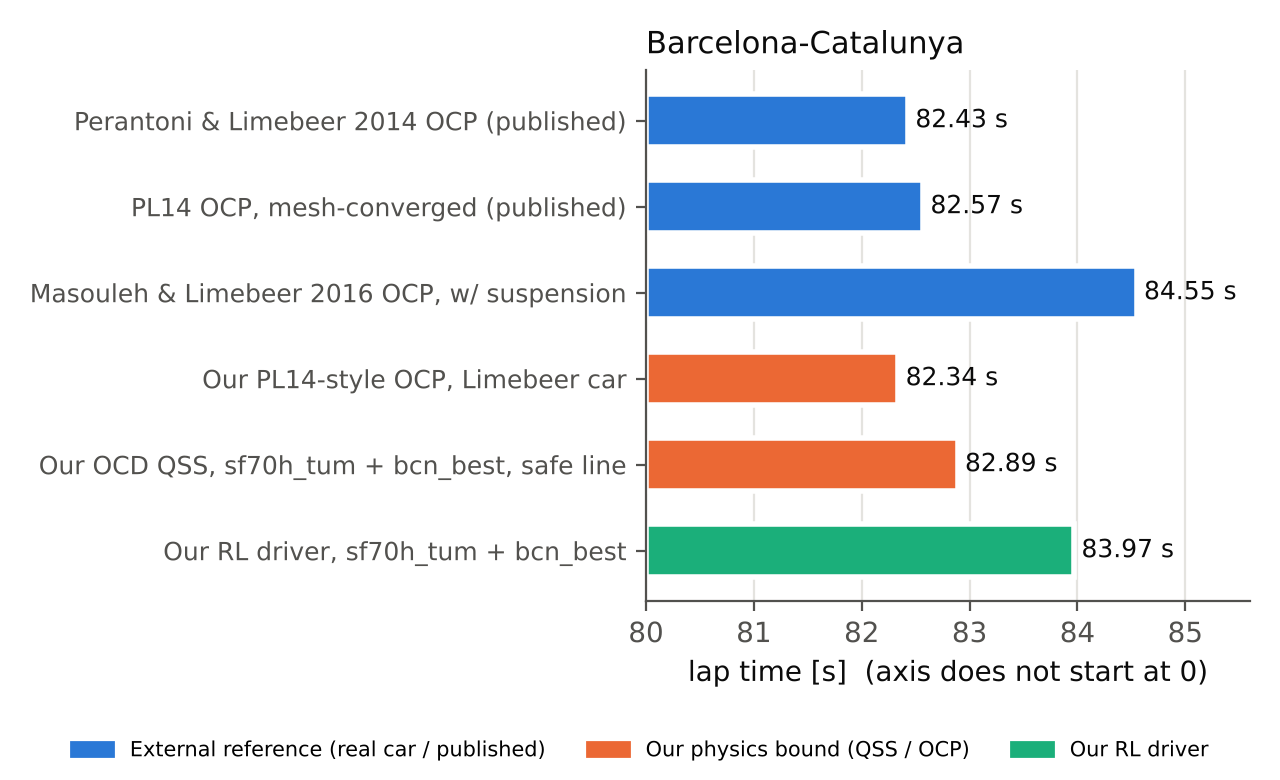
\includegraphics[width=0.9\linewidth,height=0.86\textheight,keepaspectratio]{fig/barcelona_bars.png}
\end{frame}

% 10 -----------------------------------------------------------------
\begin{frame}{Shanghai: real world vs.\ QSS vs.\ our RL driver}
  \centering
  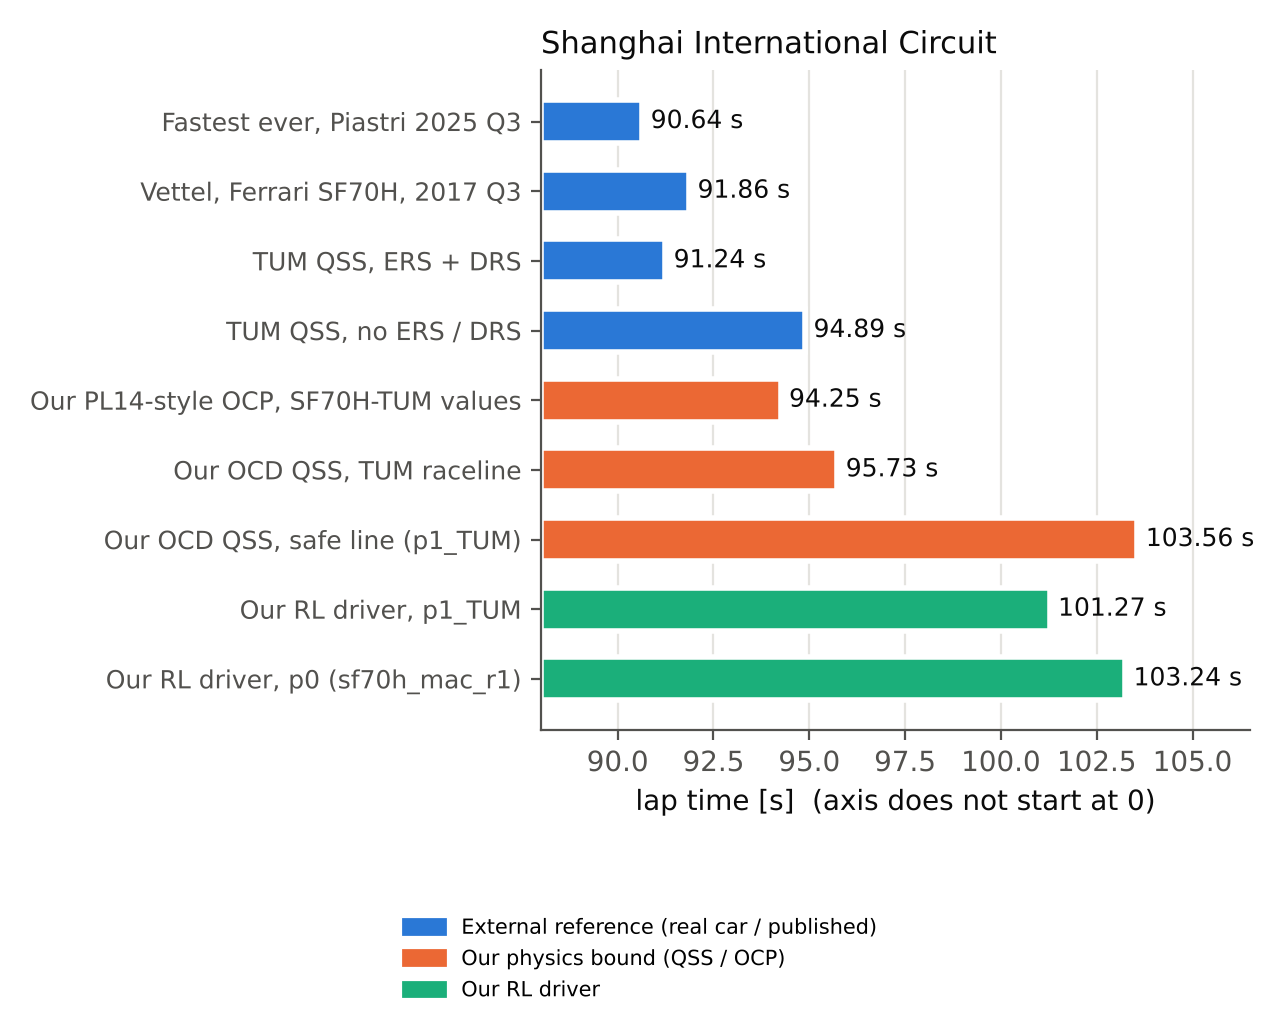
\includegraphics[width=0.9\linewidth,height=0.86\textheight,keepaspectratio]{fig/shanghai_bars.png}
\end{frame}

\end{document}
